

\chapter{Intrusion detection systems} % Main chapter title
\label{ids}
An intrusion detection system is a system which tries to determine whether a system is under attack, to detect intrusions within a system.  Intrusion detection systems are often called IDS's. Intrusions can also be called attacks or anomalies. It does this by monitoring network or system activities. One way of categorizing IDS's is based on the method of detection intrusion. The first type would be monitoring the network, these are called network-based intrusion detection systems, or NIDS. When the intrusion detection system only monitors system activities, it is called a host-based intrusion detection system, or HIDS. \cite{sans} \\
\\
Figure~\ref{fig:IDS} shows the possible placements of an IDS. It can be placed before any firewall, being the first defense of a network. This is a NIDS. An IDS can also be placed within a network. This IDS can still monitor the network but it can also monitor system activities of the workstations. An HIDS is most commonly, but not always located on the device that it monitors.
\begin{figure}[H]
\centering
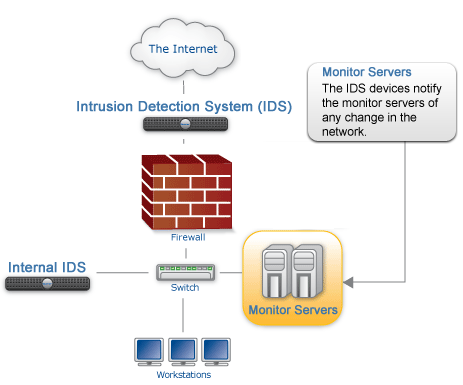
\includegraphics[width=0.9\textwidth]{Figures/idsdiagram}
\decoRule
\caption[Possible placement of IDS]{An IDS can for example be placed within the network or just before the network. \cite{ids1}}
\label{fig:IDS}
\end{figure}
\section{Host-based Intrusion Detection Systems}
Host-based intrusion detection systems are systems that monitor the device on which they are installed, or directly connected to. The way they monitor the system can range from monitoring the state of the main system through audit logs, to monitoring program execution. In this way they can be quite indistinguishable from Anti-Virus programs. \cite{sans}\\
\\
Since HIDS rely so much on audit logs, they can become limited by them. If the software that is being monitored does not provide enough information in audit logs, the IDS cannot always determine intrusions succesfully. Another issue can be the sheer volume of the audit logs. Every monitored log needs to be parsed, this means that the HIDS can have a big impact on the performance of the host system if it is installed there. \cite{Bace:1999:ID:347487} \\
\\
Another disadvantage is that any vulnerability that causes the audit files to be changed, also impacts the integrity of the HIDS. If an audit file is changed, the HIDS cannot see and detect what truly happened. \cite{Sundaram:1996:IID:332159.332161}

\section{Network-based Intrusion Detection Systems}
Network-based intrusion detection systems are placed at certain points within a network in order to monitor traffic from and to devices within the network. They operate on the same concept as wiretapping. They "tap" into a network and listen to all communication that happens.  \cite{sans} \\
\\
Using the network data instead of audit trails such as HIDS is desirable in multiple ways. One advantage is that they do not impact the performance of programs that are using the network. It is also more difficult for an intruder to attack the IDS itself. Network traffic is always visible and cannot be changed like an audit trail. The intruder could try to minimize his network activity, but the risk is lower. NIDS are also more portable than HIDS. They monitor traffic over a network and are independent of the operating system they run on.  \cite{Bace:1999:ID:347487} \\
\\
The system can analyse the traffic using multiple techniques to determine whether the data is malicious. There are two different ways to analyse the network data. The analysis can be packet-based or flow-based.\\
\\
Packet-based analysis uses the entire packet including the headers and payload. An intrusion detection system that uses packet-based analysis is called a packet-based network intrusion detection system. The advantage of this type of analysis is that there is a lot of data to work with. Every single byte of the packet could be used to determine whether the packet is malicious or not. The disadvantage is immediately obvious once we look at networks through which a lot of data passes, such as data centers. Analysing every byte is very work-intensive and near impossible to do in such environments. \cite{alaidaros2011overview} \\
\\
Flow-based analysis doesn't use individual packets but uses general aggregated data about network flows. An intrusion detection system that uses flow-based analysis is called a flow-based network intrusion detection system. A flow is defined as a single connection between the host and another device. A flow can be defined using a (source\_IP, destination\_IP, source\_port, destination\_port) tuple. However flows also contains other information. IP Flows are discussed in depth in Section~\ref{flow}. Because of the other information, flows can still contain a lot of information, even when compared to packets. Since flow data is much more compact than all the individual packets, it is much more feasable for data centers to use flow-based intrusion detection systems. \cite{alaidaros2011overview} \cite{pao2004netflow}

\subsection{Intrusion Prevention Systems}
An intrusion prevention system or IPS/IDPS is an intrusion detection system that also has to ability to prevent attacks. An IDS does not necessarily need to be able to detect attacks at the exact moment they occur, although it is preferred. An IPS needs to be able to detect attacks real-time since it also needs to be able to prevent these attacks. For network attacks these prevention actions could be closing the connection, blocking an IP or limiting the data throughput.  \cite{sans2}\\
\\
The change to requiring attacks to be detected at real time can severly impact the methods that are used to detect these attacks. For example, an IDS might give an alert even though the IDS is not certain that whatever it is alerting is actually an anomaly. An IPS needs to be certain before it can take action. Otherwise the IPS might take actions which the business employing the IPS does not want.  \cite{sans2}\\
\\
In case of a NIPS, an network-based intrusion prevention system, some advantages of being network-based are not true anymore. An NIPS needs to see all data, and preferably block network data before it reaches it's destination as seen in Figure~\ref{fig:IPS}. This means that the performance of programs using the network might be affected by the NIPS. \cite{golling2014towards}

\begin{figure}[H]
\centering
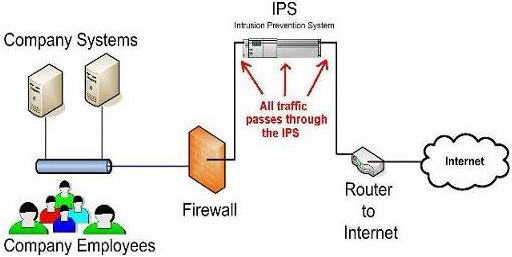
\includegraphics[width=1\textwidth]{Figures/IDS_IPS}
\decoRule
\caption[Intrusion prevention system]{An Intrusion prevention system. \cite{ips1}}
\label{fig:IPS}
\end{figure}

\section{Detection}
\label{detection}
There are mutliple different methods to detect intrusions. There are \textbf{Signature based methods} and there are \textbf{Anomaly Based} methods. Both of these methods have their own strengths and weaknesses. 
\subsection{Signature based methods}
\begin{figure}[H]
\centering
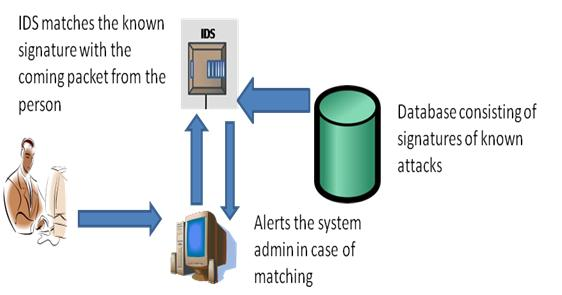
\includegraphics[width=1\textwidth]{Figures/Signature-based-Intrusion-Detection-System}
\decoRule
\caption[Signature based IDS]{An Signature-based intrusion detection system. \cite{snortImg}}
\label{fig:Signature}
\end{figure}
\noindent Signature based methods compare so called "signatures" with an existing database of signatures. An packet or flow record is decomposed into features that together construct a signature. If the signature of an incoming flow or packet matches with a signature in the database, it is flagged as malicious. Pseudocode of this can be seen below. Signature-based methods have little overhead in both computation and preprocessing as it only tries to match incoming signatures to known signatures in the database. Because it only compares signatures, it is easy to deploy within a network. The system does not need to learn what the traffic within a network looks like. \cite{methods} \\
\begin{python}
signatures = get_signatures_from_database()
while True:
    packet = get_next_packet()
    packet_signature = get_important_features(packet)
    
    if (signatures.contains(packet_signature):
        generate_alert(packet)
    else:
         # packet signature was not
         # a match with known signatures
         continue
\end{python}~\\
Signature based methods are very effective against known attacks. New attacks cannot be detected unless the database is updated with new signatures. It is also possible for attackers to avoid being caught by signature based methods, only a slight modification of the "signature" is required in order to bypass the exact matching. \cite{IPFlow}\\
\\
This could be done by trying to make the network behaviour look more like normal behaviour. For example, a botnet uses IRC communication with his master. The communication might follow certain patterns which are different from usual IRC traffic from a chat. The creator might change the botnet so that communication between the botnet and the master look similar to the usual IRC traffic. This change causes the network behaviour to be different from the signature database and not generate an alert. Updating the signature database requires a lot of technical effort, since new attacks are discovered all the time.\cite{methods} \cite{uddin2013intrusion}
\subsection{Anomaly based methods}
\begin{figure}[H]
\centering
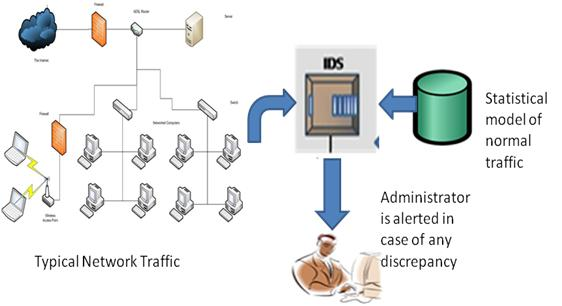
\includegraphics[width=1\textwidth]{Figures/Anomaly-based-Intrusion-Detection-System}
\decoRule
\caption[Anomaly based IDS]{An Anomaly-based intrusion detection system. \cite{snortImg}}
\label{fig:Anomaly}
\end{figure}
\noindent Anomaly based methods, also called Behaviour based methods are methods in which the IDS tries to model the behaviour of network traffic. When an incoming packet deviates from this model, it is flagged as malicious and an alert is sent. Because they use a statistical model of normal behaviour, they should be able to detect all deviations from this normal behaviour. As a result, new attacks that deviate too much from normal behaviour are detected as well. \cite{snortImg} \\
\\
Since a model of the network traffic needs to be created, the system cannot be deployed into a network and be expected to work. The system needs to learn the behaviour of the network traffic. Problems, such as generating a lot of false positive alarms, can arise when training data includes mistakes, such as misclassifications. \\
\\
Machine learning algorithms can be used as an anomaly based method. Machine learning techniques have the ability to learn from data and decide whether new data is malicous. \cite{snortImg}

\section{Existing Intrusion detection systems}
There are a lot of different intrusion detection and intrusion prevention systems on the market. Some of these systems are very expensive, others are completely open source and free. 

\subsection{Alienvault}
\textit{Alienvault} is a business that develops software to manage cyber attacks. They create SIEM solutions, Security Information and Event Management solutions. These are tools that provide methods to analyse security threats. IDS's are incorperated into SIEM's. \cite{alienvault} \\
\\
The product they make is the \textit{AlienVault Unified Security Management} (USM). USM is an all-in-one tool. USM contains a lot of tools that are required to analyse a system for cyber security threats. It contains tools that can scan and test the network for vulnerabilities. \\
\\
USM supports both host-based intrusion detection and network-based intrusion detection. It also has the option to do both full packet and netflow analysis, supporting both types of NIDS systems. \cite{alienvaultProd} \\
\\
\textit{Alienvault} works on both signature-based and anomaly-based intrusion detection. However, it is interesting to note that they are working on new strategies that can detect intrusions. Research is being done using neural networks to make intrusion detection more accurate. \cite{alienvaultIDS}

\subsection{SNORT}
Snort is an open-source network intrusion detection and prevention system. It is made to be very lightweight in use. It runs on UNIX derivatives and Windows. SNORT is the most widely used IDS worldwide and has become the in reality standard for the industry. SNORT can also operate on both packet level and IP flow level. However, SNORT uses a combination of signature and anomaly detection methods. \cite{kurundkar2012network} \\
\\
SNORT uses a system based on rules. Using rules, an administrator can configure SNORT. These rules allow for both signature and anomaly detection methods. This means that SNORT itself does not work with machine learning algorithms. However, the rules can be made using machine learning algorithms. These algorithms make rules based on which traffic is classified as normal and abnormal.  \cite{duffield2009rule} \\
\\
SNORT can, since a couple years, also be deployed as a intrusion prevention system. This is done by adding a new type of rule, a "drop" rule. A "drop" rule has higher precedence than an "alert" rule. This means that any packet that matches a "drop" rule and an "alert" rule will be dropped. \\
\\
Since SNORT is open source, the internal structure can be observed. There are several components that work together to detect abnormal behaviour and to generate output in a format that is appropriate for an intrusion detection system. \cite{kurundkar2012network}
\begin{itemize}
\item Packet sniffer and decoder
\item Preprocessors
\item Intrusion detection engine
\item Logger and alert system
\item Output modules
\end{itemize}

\noindent In Figure~\ref{fig:snort}, the structure of the SNORT components can be seen. The \textbf{packet sniffer and decoder} sniffs packets from different network interfaces. The packets are then prepared to go to the preprocessor. The \textbf{preprocessor} can already extract the most important data from packets and might even modify the data. In the \textbf{detection engine} rules are used to detect any intrusions. The rules are matched against every packet. If a packet is matched, it may be dropped or an alert can be generated, depending on the type of the rule. \\
\\
Alerts can be logged to different kinds of files. This happens in the \textbf{logger and alert system}. These could be text files or tcpdumps. The \textbf{output modules} can do different operations on the output to generate new log files.  \cite{kurundkar2012network}

\begin{figure}[H]
\centering
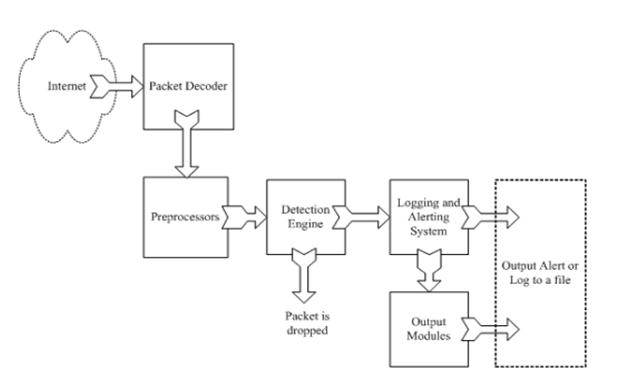
\includegraphics[width=1\textwidth]{Figures/snort}
\decoRule
\caption[The structure of the SNORT IDS]{The structure of the SNORT IDS. \cite{snortImg}}
\label{fig:snort}
\end{figure}

\subsection{MIT AI\textsuperscript{2}}
MIT is also working on methods to use machine learning to defend against cyber attacks. In their paper "\textit{AI\textsuperscript{2}: Training a big data machine to defend}", they present a new method. Their system has four components. A big data processing system, an outlier detection engine, a mechanism to obtain feedback from security analysts, and a supervised learning module.
\cite{veeramachaneniai2}\\
\\
Their system tries to combine the expertise of security experts, and the speed and ability to detect new attacks of machine learning. More specifically, they use unsupervised machine learning. They prefered to use unsupervised machine learning since labeled data is rare and attacks constantly evolve. In the system they generate their own labels and use a supervised learning algorithm with these labels. \\
\\
The \textbf{big data processing system} is a system that can extract features of different entities from raw data. The \textbf{outlier detection engine} is a system that uses unsupervised learning. It uses the features that have been found in the big data processing system. They use three different methods, density, matrix decomposition, or replicator neural networks. \cite{veeramachaneniai2} \\
\\
The output of this unsupervised system is processed and shown to a \textbf{security analyst}. The security analyst can verify or refute the output. The feedback is fed to a \textbf{supervised learning algorithm}. The supervised learning algorithm learn a model that can use this feedback to better predict whether any new event is normal or abnormal. With more feedback, the system becomes more and more correct. The flow of the system can be seen in Figure~\ref{fig:mit}. \cite{veeramachaneniai2}

\begin{figure}[H]
\centering
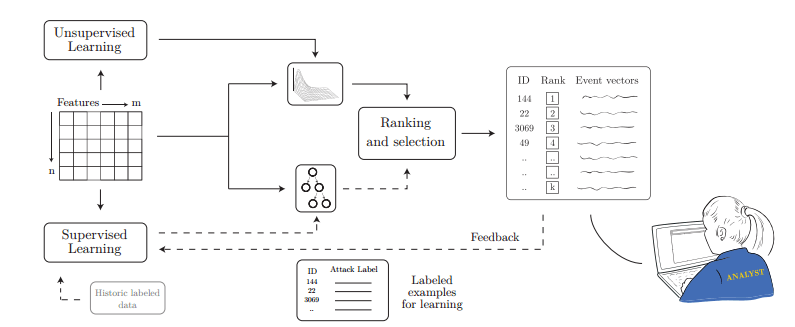
\includegraphics[width=1\textwidth]{Figures/AI2}
\decoRule
\caption[The structure of AI2 system]{The structure of AI2 system. \cite{mit2}}
\label{fig:mit}
\end{figure}

\noindent Their system has been tested by monitoring a large web-scale platform. This platform generated millions of log lines per day. The monitoring lasted three month and generated 3.6 billion log lines. They coud detect 85 percent of attacks and reduced the amount of false positives by 5 times since the previous implementation. \cite{mit2}

